\documentclass{article}
\usepackage[margin=1in]{geometry} %1 in margins
\usepackage{graphicx} %For including graphics
\usepackage[labelfont=bf]{caption} %Make float labels bold
\usepackage{subcaption}
\usepackage{amsmath}    
\usepackage{listings}% http://ctan.org/pkg/listings
\lstset{
  basicstyle=\ttfamily,
  mathescape
}
\usepackage{hyperref}
\renewcommand{\floatpagefraction}{0.95}
\renewcommand{\topfraction}{0.95}
\renewcommand{\textfraction}{0.05}
\usepackage{url}

% Define a ``Program'' float for code
\usepackage{verbatim} %Allow verbatim input for code
\usepackage{float} %Defining the Program environment
\floatstyle{boxed}
\newfloat{program}{htbp}{pgm}
\floatname{program}{Program}
\usepackage[fontsize=9pt]{scrextend}
\usepackage{color,soul}



\begin{document}
\begin{flushright}
Mehmet Duman
\end{flushright}
\begin{center}
{\Large {\bf Solution to Homework \#5---EAS 520 \& DSC 520 \& MTH 499} }
\end{center}

\textbf{\textit{Solution for Problem 1 a,b}} :
\begin{lstlisting}
f( 512, 404.2319 ) = -1059.640663 
Proccess  2, sample  1,  with f =  1.101457e+02 
Proccess  1, sample  1,  with f = -3.312653e+02 
Proccess  3, sample  1,  with f = -1.635407e+02 
Proccess  0, sample  1,  with f =  3.860226e+02 
Proccess  2, sample  2,  with f = -2.389024e+02 
Proccess  1, sample  2,  with f =  2.873286e+02 
Proccess  3, sample  2,  with f = -2.066937e+02 
Proccess  0, sample  2,  with f = -1.773359e+02 
Process 2 of 4 local min = -2.389024e+02
Process 3 of 4 local min = -2.066937e+02
Process 0 of 4 local min = -1.773359e+02
Process 1 of 4 local min = -3.312653e+02
A Ring Topology Min = -3.312653e+02          MPI Min Reduction Global Min = -3.312653e+02 
\end{lstlisting}

\textbf{\textit{Solution for Problem 1 c}} : On Stampede, I increased N sample number and  the process size (cores)=4. Result running time (Secret and Rand func)  for each proccess making single sample is converging  0.0048 sec.

\begin{lstlisting}
  N size  Min (Ring)   Min(Reduction) Entire T    Ring T     MPI T    Scrt+Rnd  Scrt&Rnd/N*size
   10, 4, -4.879420e+02, -4.879420e+02,  0.424975, 0.000063, 0.000876,  0.424036, 0.010601
   50, 4, -7.606640e+02, -7.606640e+02,  1.129642, 0.000066, 0.000869,  1.128707, 0.005644
  100, 4, -8.362344e+02, -8.362344e+02,  2.089839, 0.000061, 0.000861,  2.088917, 0.005222
  500, 4, -9.327838e+02, -9.327838e+02,  9.764632, 0.000067, 0.000943,  9.763622, 0.004882
 1000, 4, -9.312489e+02, -9.312489e+02, 19.372315, 0.000066, 0.000897, 19.371352, 0.004843
10000, 4, -9.517893e+02, -9.517893e+02,192.147944, 0.000065, 0.000920,192.146959, 0.004804
\end{lstlisting}

\begin{figure}[htb]
	\begin{center}
		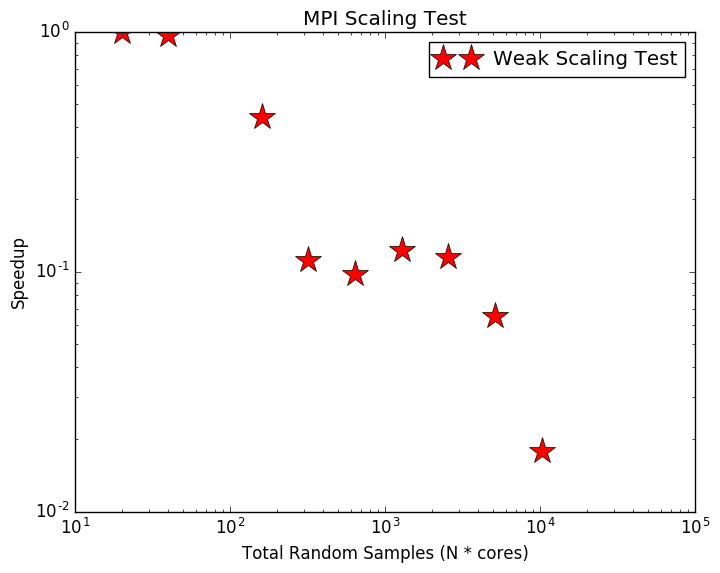
\includegraphics[width=0.8\textwidth]{hw5_p2c_1.png}
	\end{center}
\end{figure}

\begin{figure}[htb]
	\begin{center}
		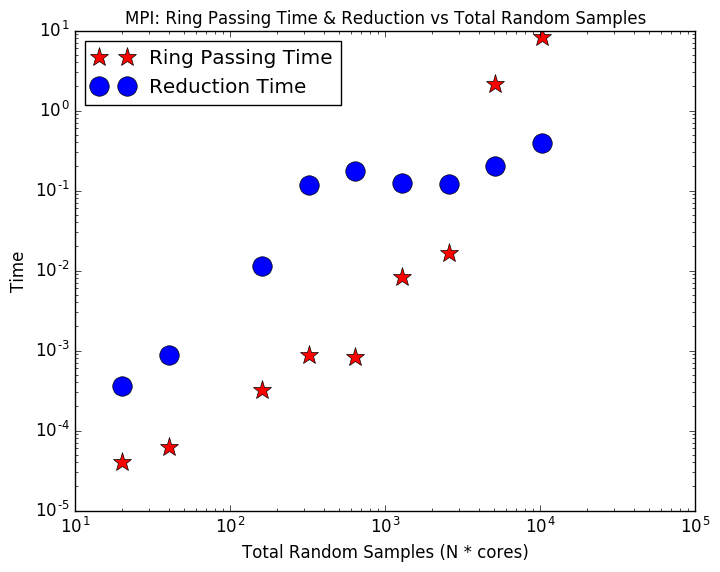
\includegraphics[width=0.8\textwidth]{hw5_p2c_2.png}
	\end{center}
\end{figure}

\begin{lstlisting}
    N   cores Min-Reduction  Entire Time   MPI Time  Secret & rand Time  Stampede output file
   4000, 1024, -1.041659e+03,  472.120754,  78.117580,  394.003174      hw5_p2d_7876445.stdou
  10000, 1024, -1.056865e+03, 1033.799760, 181.037155,  852.762605      hw5_p2d_7876648.stdou
 100000,  256, -1.059512e+03, 1931.949510,   4.449555, 1927.499955      hw5_p2d_7876775.stdou
 200000,  256, -1.055818e+03, 4095.107267, 259.863719, 3835.243548      hw5_p2d_7877455.stdou
 200000,  256, -1.058304e+03, 4095.851167, 259.731049, 3836.120118      hw5_p2d_7877521.stdou
 300000,  256, -1.059302e+03, 6142.260361, 390.724083, 5751.536278      hw5_p2d_7877590.stdou
\end{lstlisting}



\end{document}
